\chapter{Introduction}
\label{introchap}

\section{Motivation}
\sectionmark{Motivation}

\subsection{Convection in Astrophysics: Stars, Planets, \& Beyond}
\label{sct:convective_abundance}
In nature, thermal buoyancy forces primarily drive two types of flows: gravity waves and convection.
Gravity waves are driven when the fluid stratification (e.g., the atmosphere) is convectively \emph{stable}.
Convection is the manifestation of buoyancy forces in the presence of an \emph{unstable} or \emph{superadiabatic} stratification.
Convection occurs in the Earth's atmosphere, and cumulus clouds are evidence of that convection (and there is a rich literature investigating atmospheric convection, see \citet{yano2014} for a recent review).
Within the Earth, both the mantle \citep{schubert&all2001} and liquid outer core convect, respectively driving plate tectonics \citep{bercovici2003} and the Earth's magnetic dynamo \citep{christensen2011}.
Convection also occurs in more exotic astrophysical systems, including in the planes of accretion disks \citep{held&latter2018} and in the magnetospheres of giant planets \citep{thomsen&all2012}.
In short, convection is a ubiquitous process in astrophysics and geophysics.
A detailed understanding of the fundamental nature of convection is therefore crucial to understanding emergent convectively-driven phenomena in these fields.

\begin{figure}[t!]
\includegraphics[width=\textwidth]{./figs/intro/solar_convection_scales.pdf}
\caption[Images of solar granulation and supergranulation.]
{
	(left) first-light image of the solar surface from DKIST (visible light [789 nm], covering 36.5 km$^2$).
	Bright, hot granules and relatively cool, dark intergranular lanes can be observed.
	Magnetically-dominated ``bright points'' occupying the center of intergranular lanes can also be seen \citep{vankooten&cranmer2017}.
	(right) Image of the solar surface from the Dutch Open Telescope (Ca II H line [396.8 nm]).
	For a sense of scale, the small-scale speckles or ``web'' of lights in this image trace out intergranular lanes (the dark regions in the left image).
	The large-scale web of lights roughly traces out the outlines of supergranules, the largest obvious scale of convection that is observed at the solar surface.
	\label{fig:solar_convection_scales} 
}
\end{figure}



Convection in the interiors and envelopes of stars is likely the most well-studied form of convection in astrophysics.
The surface of the Sun is covered in large ($\sim$1 Mm) convective ``granules'' (see the left panel of Fig.~\ref{fig:solar_convection_scales}) which overturn on roughly a five minute timescale.
These granules lay above larger ($\sim$30 Mm) ``supergranules,'' pictured in the right panel of Fig.~\ref{fig:solar_convection_scales}, which overturn on timescales of roughly a day.
These classical convective features are visible evidence of a convection zone that occupies the outer 30\% of the Sun's radial profile \citep{miesch2005, nordlund&all2009}.
Most Main Sequence (MS) stars, including the Sun, rely on convective heat transport at one more locations within their interiors.
``Early-type'' or ``Upper-MS'' high-mass stars ($M \gtrsim 1.5 M_\odot$, where $M_\odot$ is the solar mass) have convectively unstable cores.
In these massive stars, core conditions are sufficiently hot and dense that the CNO cycle (Carbon-Nitrogen-Oxygen) is the dominant source of core hydrogen fusion.
The opacity of the stellar material, dominated by free-free interactions \citep[c.f.~Ch.~16 of][]{weiss&all2004}, is sufficiently high that the extreme CNO-fed luminosities cannot be efficiently carried by radiative processes.
Convection must therefore assist radiative conductivity to transport the stellar luminosity outward, resulting in a well-mixed convective core region in these massive stars.
The luminosity of less massive stars ($M \leq 1.5 M_\odot$) is provided by the PP-chain (proton-proton), allowing many such stars to have stable cores.
However, the cooler surface temperatures of these stars allow for phase changes of hydrogen and helium (e.g., from fully ionized to neutral) within their stellar envelopes.
These elements are the primary constituents of the stellar material, and neutral atoms greatly increase the stellar opacity through bound-free (photo effect) interactions \citep[and these effects were studied by][]{rast&toomre1993a, rast&toomre1993b}.
In solar-type stars ($1.5 M_\odot \lesssim M \lesssim 0.3 M_\odot$), the increased opacity near the stellar surface results in a convectively unstable envelope which overlies a stable, radiative interior.
In ``Late-type'', ``Lower-MS'' stars, such as M-dwarf stars, these opacity effects are sufficiently important that the star is convectively unstable throughout its full radial extent.
While stars spend the majority of their lifetimes on the MS, convection is also an important process during other evolutionary phases \citep[and I refer the reader to chapter 2 of][for a broad but brief overview of stellar evolutionary phases]{HKT}.

Convection's prevalence within stars suggests that it is a crucial process in establishing the stratification and structure of stellar interiors.
However, until recently, the insides of stars have been an unobservable region, and there has been a dearth of observations against which to test stellar convection theory.
The relatively new fields of helioseismology and asteroseismology (briefly explored in Sec.~\ref{sct:asteroseismology}) have enabled scientists to literally look inside of the Sun and stars.
These measurements allow us to put constraints upon and test the validity of stellar structure models, our assumptions about processes in stellar interiors, and our theories of convection.
Helioseismology has revealed a major discrepancy between models and observations, commonly referred to as the ``Solar Convective Conundrum,'' which I explore in detail in Sec.~\ref{sct:convective_conundrum}.
This conundrum has shown that our fundamental understanding of stellar convection is flawed.
The collection of experiments presented in this thesis were motivated by the Solar Convective Conundrum and a desire to rebuild some understanding of stellar convection from fundamental principles.

\subsection{Asteroseismology \& Helioseismology}
\label{sct:asteroseismology}
Stars are seismically active.
This seismic activity is the manifestation of complex, 3D oscillations within the star which come in two primary forms: pressure-driven ``p''-modes, and buoyancy-driven ``g''-modes.
The simplest of these modes are radial modes, in which the star experiences spherically symmetric oscillations along its radial coordinate (and the simplest of these modes is the fundamental ``breathing'' mode, whose spherical harmonic degree is $\ell = 0$, in which the star's radius expands and contracts as a whole).
Theoretically, an infinite number of (radial and nonradial) modes can be excited in a star at a given time.
The left image of Fig.~\ref{fig:asteroseismology} shows an example of the modes which can be excited within a standard model of the Sun's stratification.
Temporal frequency on the y-axis is plotted against spherical harmonic degree $\ell$, and each of the ridges in the plots is an individual mode at a specific overtone $n$.
The bottom of the diagram is filled with low-frequency, buoyancy-driven g-modes while the upper part of the diagram is filled with higher frequency, pressure-driven p-modes.

\begin{figure}[t!]
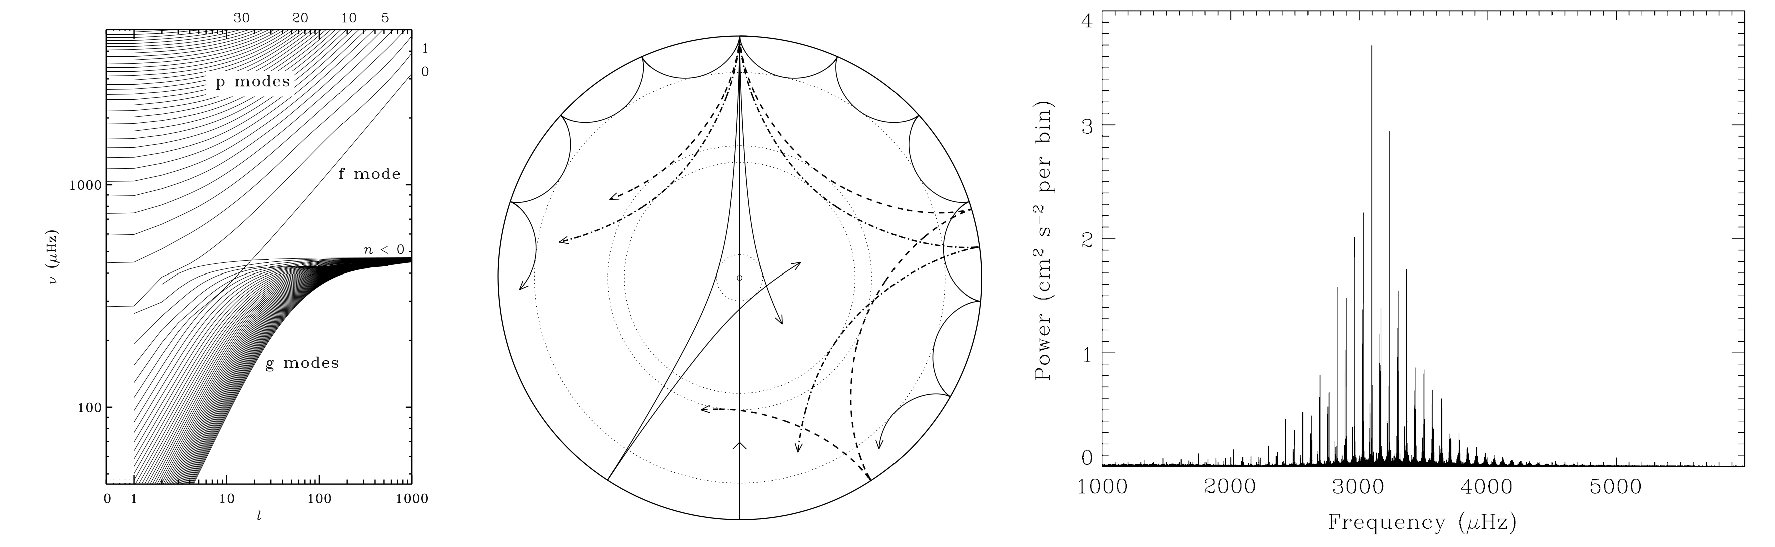
\includegraphics[width=\textwidth]{./figs/intro/asteroseismology.pdf}
\caption[Introduction to asteroseismology.]
{
	Select images describing asteroseismology, taken from Ch.~1 of \citet{aerts&all2010}.
	(left, Fig.~1.6) Allowed frequency modes in a standard solar model.
	The upper part of the diagram is filled with p modes; frequency increases with overtone $n$ and spherical harmonic degree $\ell$.
	The lower part of the diagram is filled with g modes, whose frequency decreases with overtone $n$.
	(middle, Fig.~1.7a) Propagation of rays of sound waves in a cross-section of a Sun-like star.
	Shown are rays (in increasing order of penetration depth) of spherical harmonic degree of $\ell = \{75, 25, 20, 2\}$.
	(right, Fig.~1.9) A power spectrum of radial velocity variations for 9.5 years of data of the Sun-seen-as-a-star.
	Distinct peaks corresponding to p-modes (as in the left panel) can be seen.
	\label{fig:asteroseismology} 
}
\end{figure}

As these waves propagate into the stellar interior, the stratification of the star (e.g., the changing sound speed with depth for the p-modes) causes the waves to refract and return to the surface (see the middle panel of Fig.~\ref{fig:asteroseismology}).
These waves therefore directly sample the interior stratification of the star, and the spherical harmonic degree of a given mode determines how deep it propagates before reflecting (with higher $\ell$ propagating less deeply).
Asteroseismology and helioseismology refer to the observation of complex wavefields at the stellar surface which are the summation of these waves which sample various stellar depths.
Due to the fact that stars are not spatially resolved, asteroseismology can only detect a limited number of modes.
An asteroseismic power spectrum of the Sun-seen-as-a-star is shown in the right panel of Fig.~\ref{fig:asteroseismology}.
Each of the peaks in this power spectrum correspond to one of the ridges in the leftmost panel, and the frequencies at which these peaks occur help constrain the interior structure of a given star.
Helioseismology, which is the name for the field that applies asteroseismic techniques to the Sun specifically, has access to high-resolution spatial data and can therefore probe the solar interior in more detail, including revealing the nature of mean flows like differential rotation within the Sun.
Helioseismic and asteroseismic theory, observations, and applications have respectively been covered extensively by \cite{christensen-dalsgaard2002} and \cite{aerts&all2010}.

The advent of asteroseismic science has closely paralleled that of exoplanetary science.
Early ground-based observations of stellar pulsations \cite[e.g.,][]{kjeldsen&frandsen1991, bouchy&carrier2001, bedding&all2001} have given way to datasets larger than $10^4$ stars \cite[e.g.,][]{yu&all2018, santos&all2019b} in the age of CoRoT, Kepler, and K2 data.
Another 20,000 asteroseismically-interesting targets are being observed in the TESS satellite's two-year mission \citep{schofield&all2019}.
By 2030 we expect to have observed $10^7$ pulsating red giants and $10^5$ dwarfs and subgiants \citep{huber&all2019}.
This plethora of data will teach us a great deal about the nature of stellar interiors, and will enable the accurate measurement of the ages, masses, and radii of many of these stars.
These measurements in turn facilitates studies in numerous astrophysical disciplines, including galactic archaeology and exoplanetary science.

However, inferring information about a star's structure from asteroseismic data is difficult.
Forward modeling using one-dimensional (1D) stellar structure models requires the computation of many slightly different models to produce a model which lines up well with a given set of observations, and backwards modeling is in and of itself a difficult proposition.
For a more complete discussion of the difficulties inherent in asteroseismic techniques, I refer the reader to Chs.~1.4 \& 4.1 of \citet{bellingerT2018}.
Regardless, 1D stellar structure models consistently fail to reproduce some aspects of asteroseismic observations; one such example is that models and observations frequently do not align in the highly supercritical surface layers of solar-like stars \citep[as discussed in][]{jorgensen&weiss2019}.
Some of the known deficiencies of stellar structure models are described by \cite{buldgen2019}, and of particular interest in the context of this thesis are their handling of three-dimensional (3D) dynamical phenomena like convection.
In order to improve these models, we must improve how stellar structure codes handle convection.
By improving convective models and stellar structure models, we can better take advantage of the exponential rise in asteroseismic targets that has occurred---and continues to occur---in recent years.



\subsection{The Solar Convective Conundrum}
\label{sct:convective_conundrum}
Recent observations have revealed that we lack a fundamental understanding of the convective dynamics in the Sun's convective envelope.
Helioseismic observations \citep{hanasoge&all2012, greer&all2015} have reported detections of convective velocity magnitudes which are different by a factor of 100.
Despite these disagreements, one way in which these observations broadly agree with one another and broadly agree with measurements of solar surface velocities \citep{hathaway&all2015} is that solar convection has an unexpected absence of velocity at large spatial scales.
In short, we do not observe large-scale ``giant cells'' driven by buoyant motions deep in the solar convection zone in helioseismic (left panel of Fig.~\ref{fig:conv_conundrum}) or surface velocity (right panel of Fig.~\ref{fig:conv_conundrum}) measurements.
These measurements, and the absence of giant cells, constitute the Solar Convective Conundrum.
Two primary hypotheses currently aim to explain the absence of giant cells: 
\begin{enumerate}
\item The ``entropy rain'' hypothesis, and
\item The rotationally constrained solar interior hypothesis.
\end{enumerate}
I will briefly describe each of these hypotheses below.

\begin{figure}[t!]
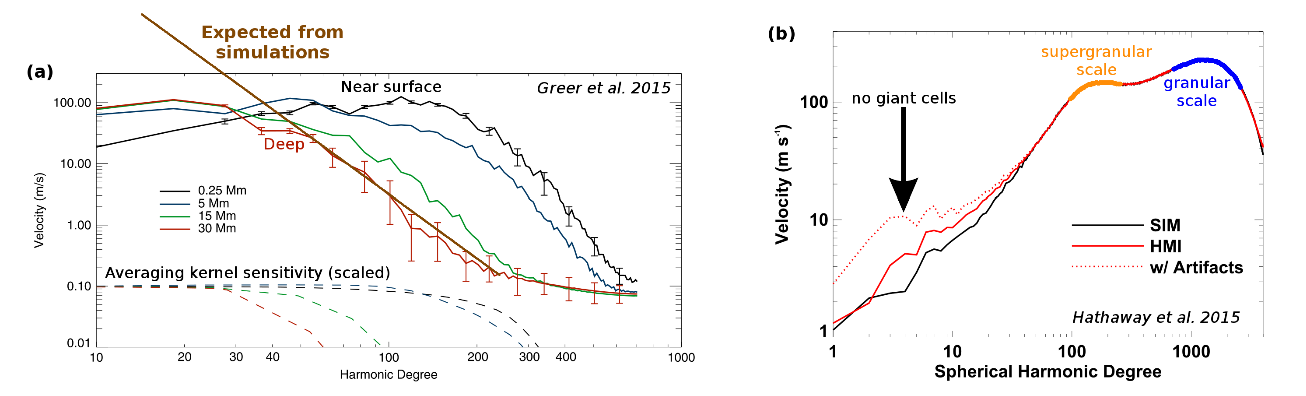
\includegraphics[width=\textwidth]{./figs/intro/conv_conundrum.pdf}
\caption[The convective conundrum.]
{
	\citep[a, annoted Fig.~3 from][]{greer&all2015} Ring-diagram helioseismic observations of the solar velocity power spectrum at various depths.
	Here, velocity power decreases toward larger scales, unlike what is expected from simulations.
	\citep[b, annotated Fig.~8 from][]{hathaway&all2015} A spectrum of horizontal velocities at the solar surface, obtained using line-of-sight Doppler velocities.
	The length scales of surface granules and deeper supergranules appear as distinct features, but the hypothesized giant cells are not observed at low wavenumber.
	\label{fig:conv_conundrum} 
}
\end{figure}

First suggested by \cite{spruit1997}, the entropy rain hypothesis suggests that many theories over-predict the importance of upflows in solar convection.
Instead, perhaps \emph{downflows} are the predominant mechanism responsible for carrying the solar luminosity across the solar convection zone.
Recent theory and simulations \citep{brandenburg2016, kapyla&all2017}, including some of my own work (Ch.~\ref{ch:alb19}), suggest that small, intense downflows can indeed traverse the entire convection zone intact and may be more important than upflows in solar-like convection.
A slice of the traditional view of the solar interior is shown in the left panel of Fig.~\ref{fig:conundrum_solns}, and the solar interior under the entropy rain hypothesis is shown in the middle panel.

Meanwhile, the rotationally constrained interior hypothesis suggests that Coriolis forces dominate force balances in the deep solar convection zone, and that these prevent giant cells from being generated.
Simulations by \cite{featherstone&hindman2016a, featherstone&hindman2016b} show that as convective flows become more rotationally constrained, the peak of convective velocity power shifts to smaller length scales.
A model of the solar convection zone under this hypothesis is shown in the right panel of Fig.~\ref{fig:conundrum_solns}.
However, rotational effects on simulations can be hard to quantify; some simulations which nominally rotate at the solar rate show \emph{anti-solar} differential rotation \citep{gastine&all2014}, and other rotationally constrained simulations exhibit Jupiter-like bands \citep{brun&all2017}.
Regardless, current results and hypotheses suggest that the interplay between downflows and rotational effects must be better understood in stellar convection.
In Ch.~\ref{ch:ro_p19}, I make an effort to better understand how to control the degree of rotational constraint in simulations.

\begin{figure}[t!]
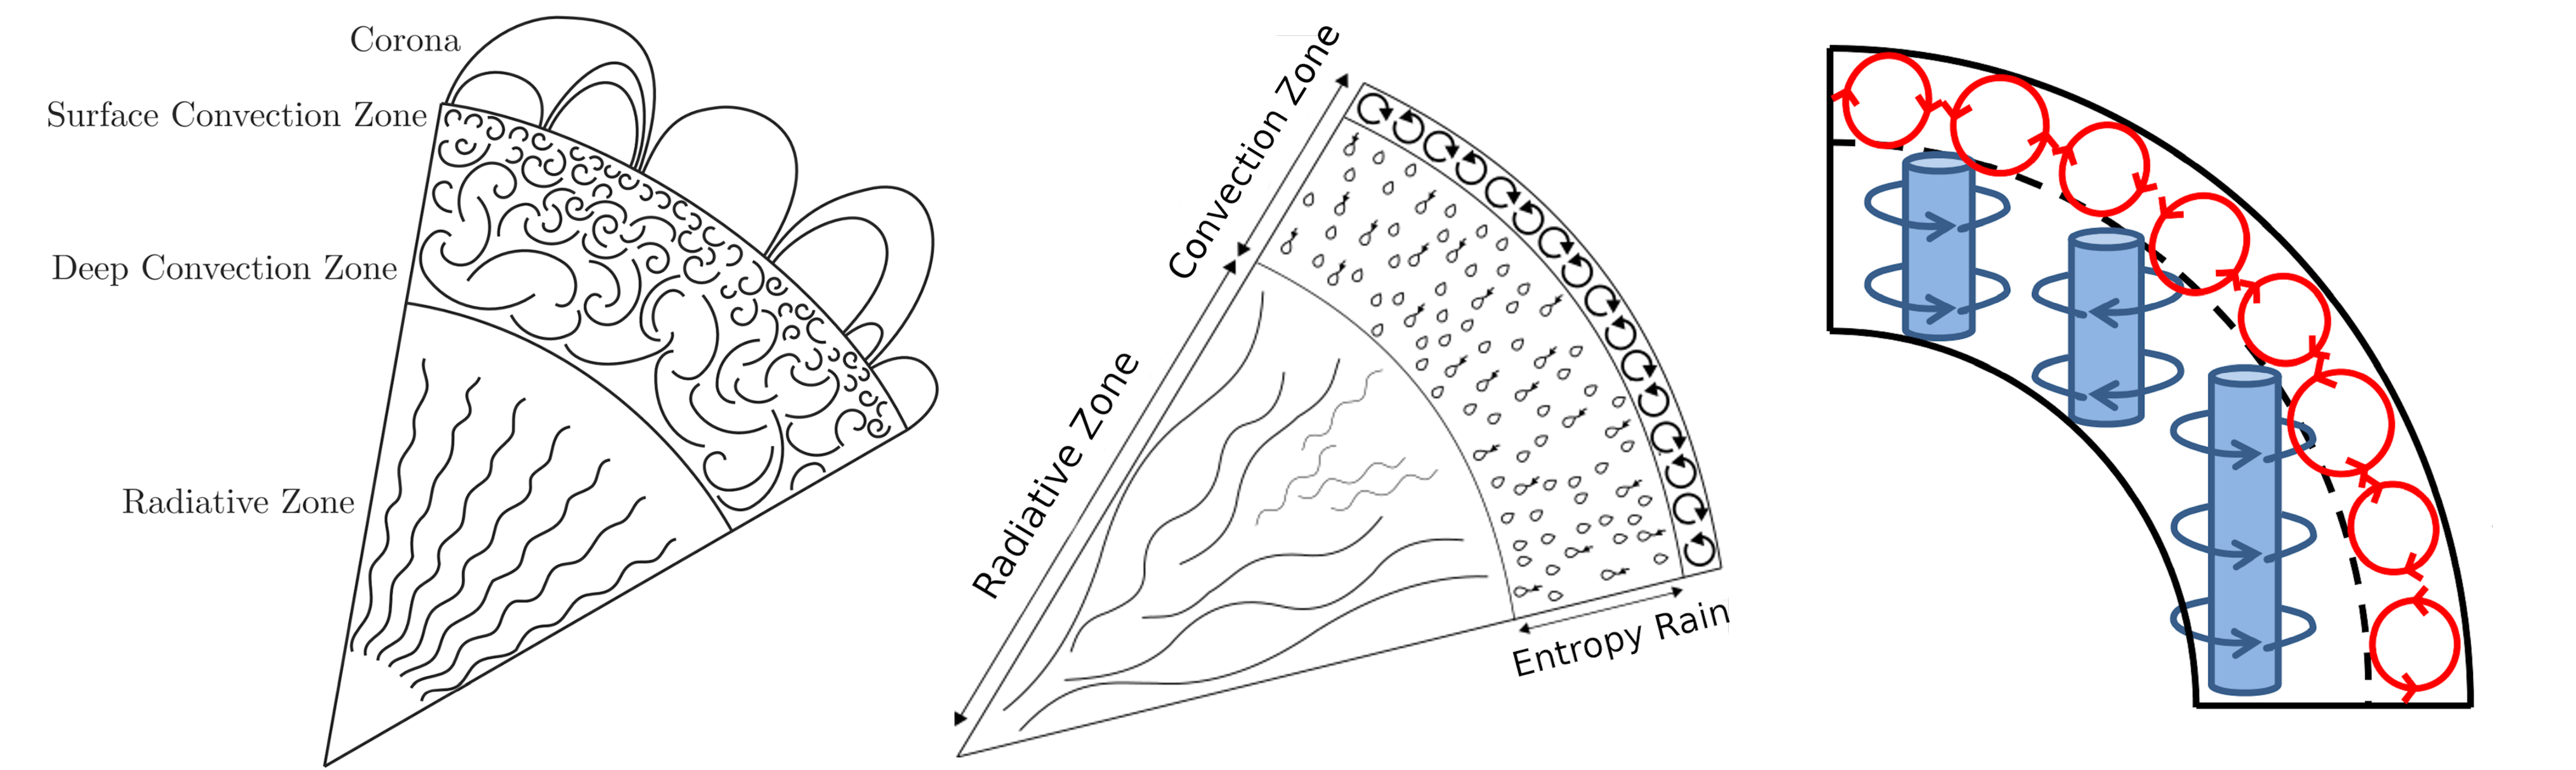
\includegraphics[width=\textwidth]{./figs/intro/conundrum_explanations.pdf}
\caption[Schematics of hypotheses that solve the convective conundrum.]
{
	(left, image courtesy of Daniel Lecoanet) The classic model of the solar interior.
	A deep radiative zone lies beneath a convective envelope; within the convective envelope, large convective cells are driven at the base, small cells are driven near the surface, and there is a gradient of cell sizes with increasing radius.
	(middle) The entropy rain picture of the solar interior.
	Beneath a thin surface convection zone, downflows or ``raindrops'' carry the solar luminosity from the solar surface to the base of the convection zone. 
	\citep[right, Fig.~3c of][]{featherstone&hindman2016b} The picture of the solar convection zone with a low-Rossby number, rotationally constrained interior.
	Rotational constraint increases with depth; below a certain depth, rotation dominates and convective cells give way to columns aligned with the global solar rotation.
	\label{fig:conundrum_solns} 
}
\end{figure}


\section{Perspectives on Studies of Convection}
Historically, experiments into the nature of convection have come from two distinct lines of motivation.
As is the case of the studies presented in this thesis, many studies into convection are motivated by the prevalence of convection in the natural world and a desire to understand convectively-driven processes.
The second line of motivation stems from turbulence research, because convective experiments are ideal systems in which to study buoyantly driven turbulent flows.
These two motivations have led to a large variety of studies into the nature of convection, which I will attempt to briefly summarize in the following sections.
Generally, studies of turbulent flows have focused on simple convective laboratory experiments or simulations in the Boussinesq regime, whereas astrophysically or geophysically motivated studies range from the same simple experimental setups to complex magnetohydrodynamic, global ``dynamo'' simulations in spherical domains.

\subsection{\RB convection}
The first controlled laboratory experiments of convection (or, a fluid layer heated from below and cooled from above) were performed by B\'{e}nard in 1900.
However, the first theoretical description of such a convective layer was performed by \citet{rayleigh1916}, who first derived the fundamental control parameter of convection: the Rayleigh number,
\begin{equation}
\text{Ra} = \frac{\alpha g L^3 (\Delta T)}{\nu \chi},
\label{eqn:rayleigh_number}
\end{equation}
where $\alpha$ is the coefficient of thermal expansion ($\alpha \equiv \partial \ln \rho / \partial T$, for the density $\rho$ and temperature $T$), $g$ is the gravitational acceleration, $L$ is the depth of the fluid layer, $\Delta T$ is the temperature difference across the fluid layer, and $\nu$ and $\chi$ are respectively the viscous and thermal diffusivities.
Colloquially, Ra can be thought of as the ratio of buoyant convective driving to viscous dissipation, and the pioneering work of these scientists in the field are the reason that Boussinesq thermal convection is widely known as \RB convection (RBC).
Together with geometric factors (the size and shape of the experimental domain), boundary conditions, and the Prandtl number (Pr = $\nu/\chi$), Ra fully describes a convective system.
Ra is an ideal control parameter for a convective system, because it is a straightforward knob for convective driving: above some ``critical value,'' $\text{Ra} > \text{Ra}_{\text{crit}}$, a fluid layer should convect, and the more ``supercritical'' an experiment is (or, the larger $S = \text{Ra}/\text{Ra}_{\text{crit}}$ is), the more turbulent the convection should be.
Furthermore, the value of $\text{Ra}_{\text{crit}}$ is independent of $\text{Pr}$ and is therefore independent of the specific fluid used in a convective experiment (e.g., in air Pr = 0.7 and in water Pr = 7).

\begin{figure}[t!]
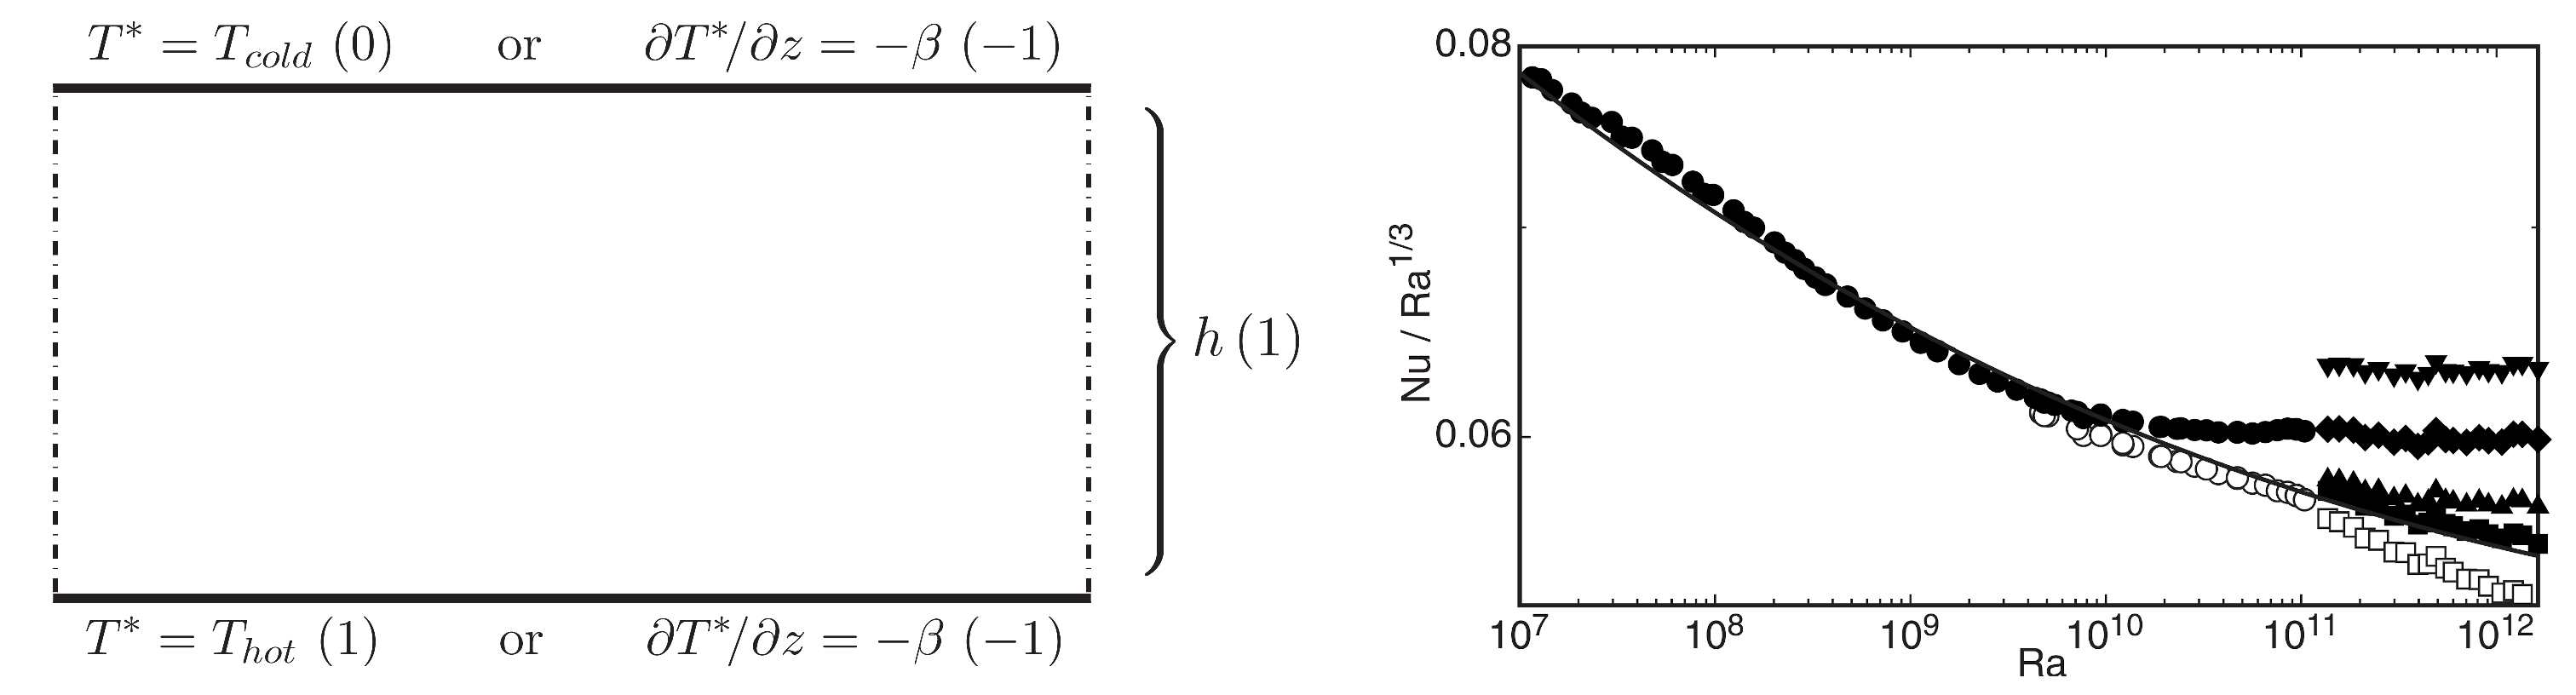
\includegraphics[width=\textwidth]{./figs/intro/rayleigh_benard_description.pdf}
\caption[A description of \RB convection studies.]
{
	\citep[left, Fig.~1 of][]{johnston&doering2009} A simple schematic of the \RB problem.
	A hot plate sits below a cold plate, and either the flux (temperature gradient) or the temperature is fixed at each plate to maintain the convective instability.
	\citep[right, Fig.~4 of][]{ahlers&all2009} A compensated scaling plot of Nu vs.~Ra.
	Here, the value of Nu is divided by the expected scaling, Ra$^{1/3}$.
	The downward trend at low Ra means that, if you assume Nu$\,\propto\,$Ra$^{\alpha}$, the value of $\alpha < 1/3$ (and $\alpha \approx 2/7$ has been frequently used in the literature).
	However, at high values of Ra, when the trend flattens, it suggests that a Ra$^{1/3}$ law is a good description.
	\label{fig:rayleigh_benard_description} 
}
\end{figure}

Historical reviews of the development of studies of RBC can be found throughout the decades in e.g., \citet{busse1978, siggia1994, ahlers&all2009}.
In the simplest of terms, much of the research into RBC focuses on the behavior of heat transfer across a convective domain, quantified by the nondimensional Nusselt number (Nu),
\begin{equation}
\text{Nu} = \frac{\text{Evolved Convective Flux}}{\text{Comparison Hydrostatic Flux}} = \angles{\frac{w T - \chi \partial_z T}{|\chi \Delta T / L|}},
\end{equation}
where $w$ is the vertical velocity, and $T$ is the temperature field, and $\angles{}$ are a volume average over the convective domain.
The key historical question that has been asked is: how does Nu scale as Ra and Pr are changed?
A schematic of the RBC setup and a sample scaling plot of Nu vs.~Ra are shown in Fig.~\ref{fig:rayleigh_benard_description}.
The earliest theoretical description developed by \citet{malkus1954} asserts that the boundary layers of convective domains are always in a marginally stable state, and thus when the Rayleigh number is defined with $L = \delta$, the boundary layer thickness, it should always have a value of Ra$_{\text{crit}}$.
This argument suggests that $\delta \propto \text{Ra}^{-1/3}$.
Assuming that the convection develops an isothermal interior and that the full temperature jump across the domain occurs in the boundary layers, we can substitute $L = \delta$ in the definition of Nu, and we retrieve a classical scaling law of $\text{Nu} \propto \text{Ra}^{1/3}$.
This scaling, or similar scalings have been seen in experiments for decades.



More recently, in \citet{grossman&lohse2000} and following papers, a unifying theory of scaling behavior has been developed that is based around the dissipation of kinetic and thermal energy in convective experiments.
The dissipation for each of these energies is split into a bulk and boundary layer component, as it is assumed that different force balances dominate the equation of motion in the bulk or boundary layers.
It is next assumed that, for each type of energy, \emph{either} the bulk \emph{or} boundary layer is predominantly responsible for dissipation of that type of energy.
Scaling laws are then determined by where in the domain each type of energy is primarily dissipated, and this results in four regimes in parameter space (e.g., where kinetic energy is dissipated in the boundaries but thermal is dissipated in the bulk, and other permutations).
A great number of studies have historically sought out the so-called ``ultimate regime'' of convection, which is the regime in which boundary layer dissipation is unimportant compared to the bulk.
Some authors have recently claimed to have achieved this ultimate regime \citep[see e.g.,][]{zhu&all2018}, but this is still a point of contention in the community.
This theory, and a comparison to experimental and numerical results, are described in detail in the review of \citet{ahlers&all2009}.

\subsection{More Realistic Geophysical and Astrophysical Experiments}
While modern and historical studies of RBC have allowed the community of convective modelers to understand convective experiments to a much greater degree, they do not contain all of the ``ingredients'' which are important to astrophysical or geophysical convection.
Numerous studies exist which aim to understand these additional complexities, ranging from studies which essentially study RBC with one extra component to studies with realistic radiative transfer, magnetism, etc.

The effects of rotation, and to a lesser extent magnetism, have been studied in the RBC context in great detail.
\citet{plumley&julien2019} provide an excellent overview of these fields.
In general, the presence of global rotation or a strong background magnetic field suppress convection, and thus increase the value of Ra$_{\text{crit}}$.
At low supercriticalities above Ra$_{\text{crit}}$, rotational (e.g., Coriolis) or magnetic forces dominate the convective flow balances.
As $S$ is increased, these forces become less important until eventually convection behaves almost indistinguishably from its nonrotating or nonmagnetic forms.
Theoretical descriptions of these models often focus on understanding scaling laws in the rotationally- \citep[e.g.,][]{julien&all2012} or magnetically- \citep[e.g.,][]{cioni&all2000} dominated regime.
A sample of the manner in which scaling laws change in the rotationally- and magnetically-constrained regimes can be seen in Fig.~\ref{fig:rotation_mhd_rayleigh_benard}.
In this thesis (Ch.~\ref{ch:ro_p19}), we focus on the effects of rotationally-influenced convection in stratified atmospheres.

\begin{figure}[t!]
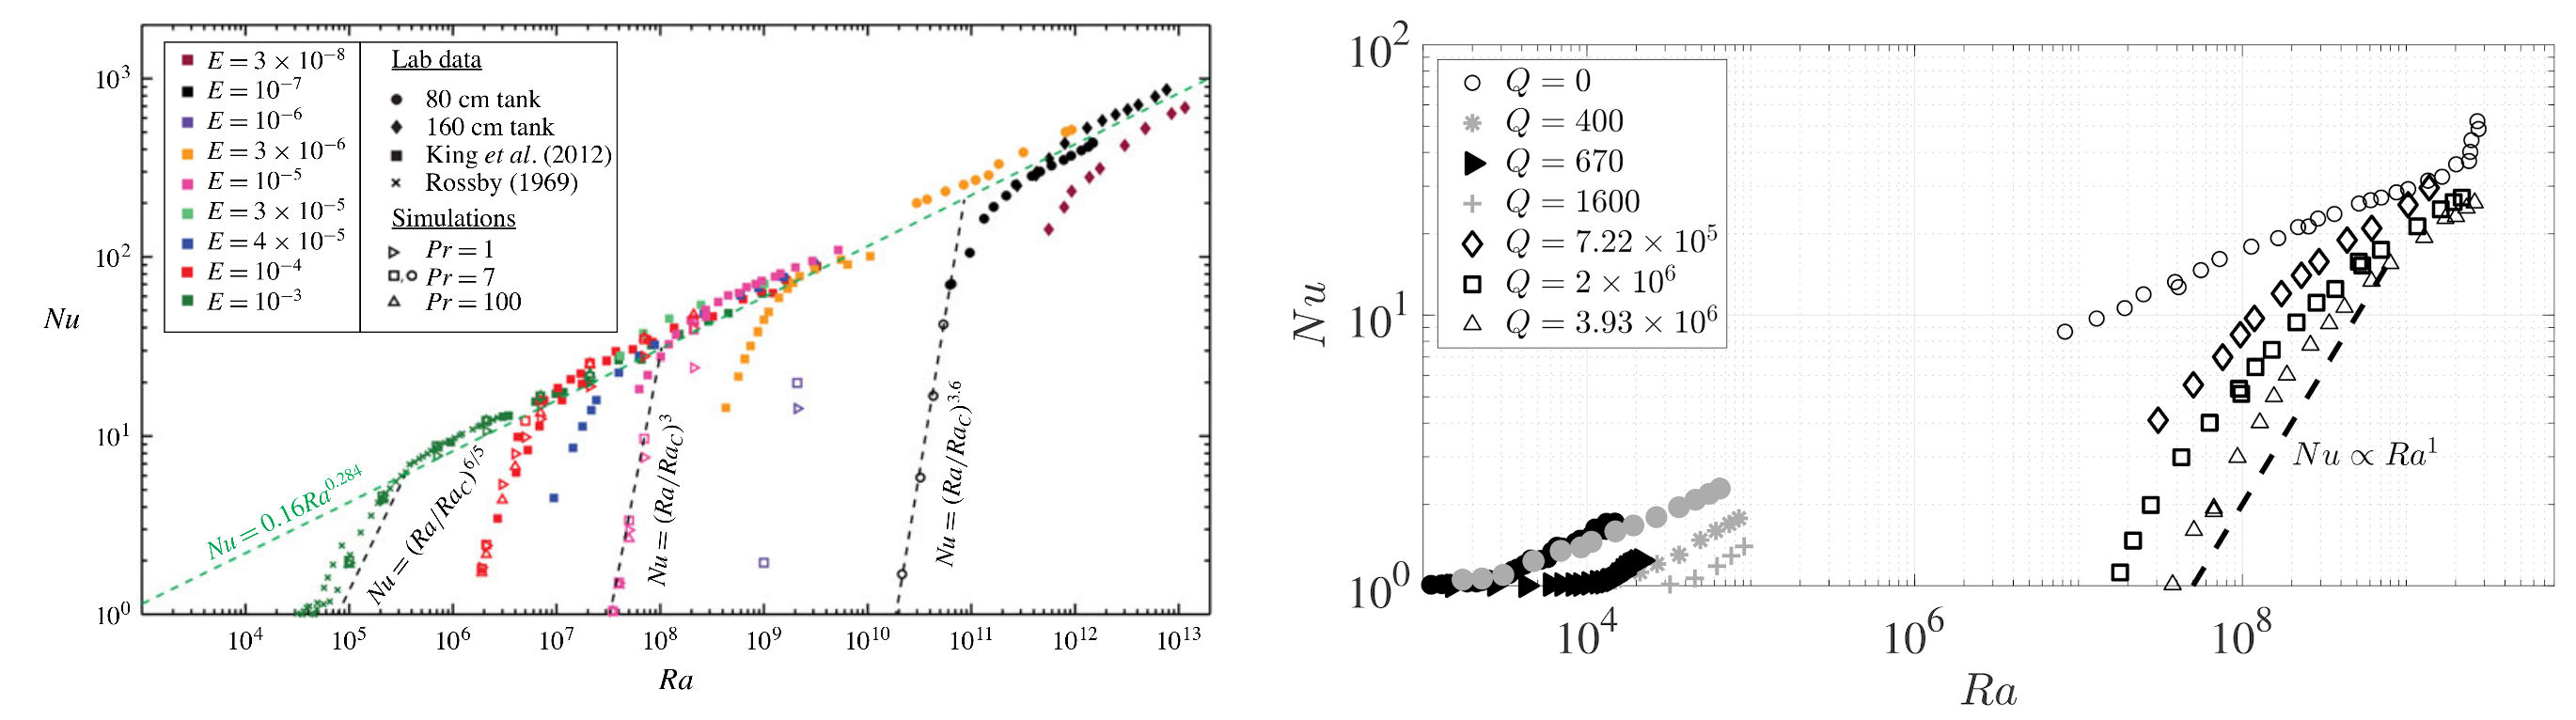
\includegraphics[width=\textwidth]{./figs/intro/rotation_mhd_rayleigh_benard.pdf}
\caption[Modification of Nu vs.~Ra in rotating RBC and magnetoconvection.]
{
	\citep[left, Fig.~1 of][]{julien&all2016} Nu vs.~Ra scalings of rotating \RB convection.
	The green line shows the rough scaling of Nu vs.~Ra in the nonrotating regime.
	Below that line, rotationally constrained experiments can be seen.
	Due to rotational stabilization of convection, these experiments have a higher value of Ra$_{\text{crit}}$ (and therefore convection ``turns on'' further to the right).
	As rotational constraint becomes less important, these simulations rapidly scale upwards towards the nonrotating values, and then follow those values once rotational constraint is not important.
	\citep[right, Fig.~4 of][]{plumley&julien2019} The same, but for magnetoconvection.
	This parameter space is significantly less well-explored.
	\label{fig:rotation_mhd_rayleigh_benard} 
}
\end{figure}


Outside of the realm of RBC, the field of convective research is less systematic and focused.
Atmospheric density stratification is one key ingredient of convection in geophysical and astrophysical applications.
The simplest stratified convection studies utilize a polytropic stratification, which has a linear temperature profile and is therefore at least somewhat comparable to RBC.
The first study which determined how to find Ra$_{\text{crit}}$ in a polytropic atmosphere was \citet{unnoetall1960}, but the first dynamical simulations of polytropic convections could not be performed until those of \citet{graham1975}.
These early works focused on similar questions to those studied in the RBC community (how does Nu behave as Ra increases?) but were limited to a very small range of supercriticalities.
Subsequent studies into polytropic convection \citep[e.g.,][]{hurlburt&all1984, cattaneo&all1991} have often focused on the morphology of overall convective flows, forces responsible for those morphologies, and the emergent nonlinear phenomena.
This trend has continued as complicating physics were added in addition to stratification (e.g., rotation in \citet{brummell&all1996, brummell&all1998}, stably stratified layers in \citet{hurlburt&all1986, singh&all1995, brummell&all2002}, or magnetism/dynamo action in \citet{nordlund&all1992, brandenburg&all1996, tobias&all1998}).
A visualization of one of dynamics in one of these simulations is shown in the left panel of Fig.~\ref{fig:complex_simulations}.

As the capabilities of supercomputers have expanded, so too have the complexity of convective simulations.
Modern ``dynamo simulations'' examine the evolution of rotating magnetohydrodynamic convection in spherical domains and have produced fascinating phenomenon.
These dynamo simulations regularly produce self-consistent differential rotation \citep{strugarek&all2018}, ``wreaths'' of magnetism \citep[][and visualized in the middle panel of Fig.~\ref{fig:complex_simulations}]{brown&all2010, brown&all2011}, magnetic cycles \citep{brown&all2011}, and more phenomenon.
These emergent phenomena parallel observed phenomena on the Sun and suggest that our fundamental understanding of the Sun's dynamo (that it is driven by turbulent motions in the convective zone) is correct.
Unfortunately, these simulations are difficult to run and are are extremely complex.
As a result, these simulations serve a role similar to observations: it is easy to see what phenomena they produce, but it is hard to understand and predict how those phenomena occurred.

\begin{figure}[t!]
\vspace{0.25cm}
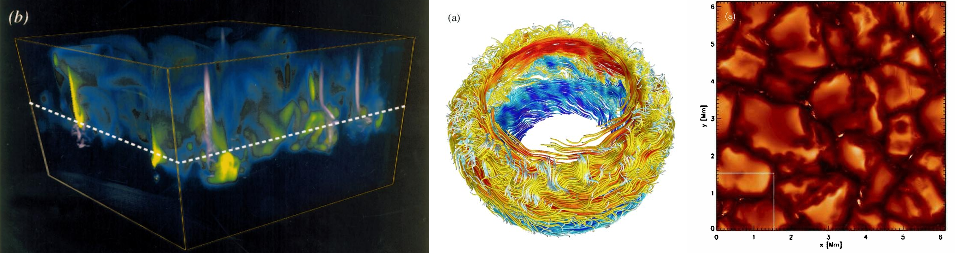
\includegraphics[width=\textwidth]{./figs/intro/complex_simulations.pdf}
\caption[Visualizations of modern simulations of astrophysical convection.]
{
	\citep[left, Fig.~2b of][]{tobias&all1998} A visualization of enstrophy (purple) and magnetic field (blue, yellow) in a stratified simulation where a convecting region lies above a stable region.
	\citep[middle, Fig.~2a of][]{brown&all2011} A visualization the azimuthal magnetic field in a spherical dynamo simulation (red is positive, blue is negative).
	\citep[right, Fig.~6a of][]{rempel2014} Intensity of light near the surface of a realistic, solar surface simulation.
	\label{fig:complex_simulations} 
}
\end{figure}


While dynamo simulations are complex due to their geometry and scale, they often do not contain the most ``realistic'' physics.
Small scale ``local'' simulations with realistic radiative transfer strikingly visually resemble solar surface convection and sunspots \citep{stein&nordlund1998, rempel&all2009, stein&nordlund2012, rempel2014}.
These simulations visually resemble solar surface convection so convincingly (see the right panel of Fig.~\ref{fig:complex_simulations}) that the raw data of e.g., \cite{rempel2014}'s simulations are being used directly as high-resolution observations of solar convection \cite[see e.g.,][and others]{vankooten&cranmer2017, shchukina&trujillo2019}.
Whether or not such a practice is wise is beyond the editorial domain of this thesis, but as a numericist I generally advise caution in directly viewing the outputs of simulations as comparable to observations.

Outside of simulations, convective experiments have become increasingly complex in recent years.
Rotating magnetoconvection experiments have been performed in cylindrical cases using liquid gallium \citep{aurnou&all2018}.
Distributed dye and light have been used to model driving of convection by internal heating, as in the interior of stars \citep{bouillaut&all2019}.
Small-scale spherical convecting plasma domains have even been produced \citep{koulakis&all2018}.
All of these experiments provide excellent opportunities to better understand convection and give us excellent models against which to compare and benchmark simulations.
These experiments are shown briefly in Fig.~\ref{fig:convective_experiments}

\begin{figure}[t!]
\vspace{0.25cm}
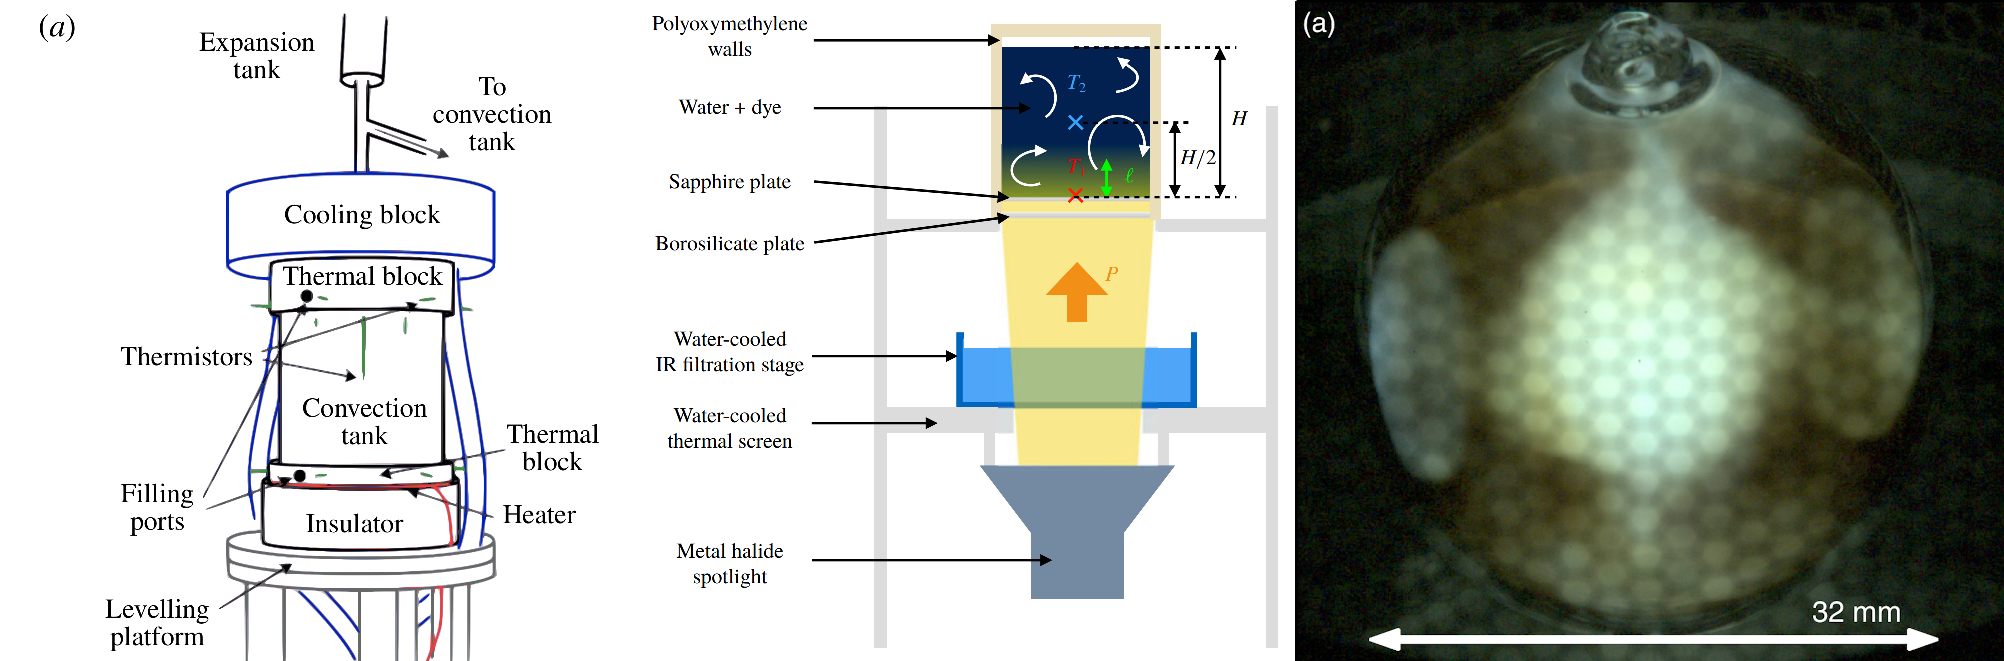
\includegraphics[width=\textwidth]{./figs/intro/convective_experiments.pdf}
\caption[Modern convective laboratory experiments.]
{
	\citep[left, Fig.~1a of][]{aurnou&all2018} A cylindrical experiment filled with liquid gallium in which rotating magnetoconvection can be studied.
	\citep[middle, Fig.~1a of][]{bouillaut&all2019} An experiment in which internally heated convection can be studied.
	The dye in the water absorbs the light, heating the water throughout the tank, and driving convection.
	\citep[right, Fig.~3a of][]{koulakis&all2018} An experiment in which pycnoclinic acoustic forces contain a hot plasma sphere at the center of a bulb.
	\label{fig:convective_experiments} 
}
\end{figure}


The ultimate goal of convective models in the context of solar or stellar convection is to understand how the solar dynamo operates so that we can eventually predict its behavior.
Modern studies have proven that we have the computational resources to create impressive simulations which strongly resemble the Sun.
It is now crucial to simplify our simulations to conduct \emph{experiments} in which we study how specific pieces of convection behave \citep[such as in the studies of tachocline interactions of][]{wood&brummell2018}.
Through the knowledge gained in more focused studies, we can better predict the results of global simulations.
This in turn will help us build better dynamo models to help predict dynamo action in geo- or astrophysical convection.


\subsection{Mixing Length Theory \& Stellar Structure Models}
While the first analytical description of convection was performed by \citet{rayleigh1916}, the earliest formulation of a simple mixing length theory was derived by \citet{prandtl1925}.
These were later expanded by \citet{vitense1953} and \citet{bohm-vitense1958} into the predecessor to most formulations of stellar mixing length theory (MLT) used today.
Modern MLT has many branches, but the one described in Chapter 14 of \citet{weiss&all2004} and earlier versions of Cox \& Giuli's book provide an excellent and fundamental description of MLT.

MLT serves as a one-dimensional (1D) description of complex three-dimensional convective motions.
MLT assumes that, at a given stellar radius, the complex distribution of convective elements present can be modeled as an average convective element whose properties depend on the star's local structure.
Each of these elements is assumed to travel the ``mixing length'' before depositing its thermodynamic signature into the surrounding matter and losing its identity.
As a result, hot elements transport warm material upward some mixing length, cold elements transport cold material downward some mixing length, so on average heat is transported outward and a 1D convective flux can be constructed.
While MLT is obviously an over-simplification of convective processes, it works qualitatively, and until recently it showed few noticeable disagreements with the observations available.
More importantly, there is no other 1D description of convection that is widely accepted by the community, so MLT is all that 1D modelers have available to work with.

State-of-the-art stellar structure models are produced by 1D codes like MESA \citep{paxton&all2011}, which depend on convective parameterizations like MLT.
Stellar structure models produced with MLT have aligned well with helioseismic observations for quite some time \citep{christensen-dalsgaard&all1996}, and disagreements between models and observations are generally less than a few percent \citep{serenelli&all2009}.
One particular area of weakness for these models has been problems due to ``near-surface effects'' \citep{kjeldsen&all2008}.
In short, MLT assumes that all convective flows are in perfect pressure equilibrium with their surroundings.
This assumption breaks down in the high-Mach number, highly superadiabatic surface layers of solar-like stars.
Recent efforts \citep{jorgensen&weiss2019, mosumgaard&all2020} have successfully coupled 1D stellar evolution models with thin, near-surface, 3D convective shells.
These studies have found that their realistic treatment of the highly adiabatic surface layers (via 3D convective simulations) do indeed reduce errors in asteroseismic frequencies between models and observations.
However, ``patching'' together 1D and 3D simulations in this manner is not a thorough solution to this problem.
3D simulations are expensive, and it is infeasible to recompute 3D simulations at each timestep in a 1D stellar structure model over the course of a star's lifetime.
Regardless, these results suggest that MLT fails to describe stellar convection, so our community must either improve models or learn how to cleverly and generally couple 1D models and 3D simulations.

One additional weakness of 1D stellar structure models is that they often neglect complicating effects like magnetism and rotation.
MESA has incorporated diffusion of angular momentum to enable at least some basic models of rotating stars \citep{paxton&all2013}.
Furthermore, recent theoretical and numerical studies have sought to understand how well mixing length theory describes rotating convection \citep{BDLithwick2014, currie&all2020}, and have shown good agreement between modified rotational MLTs and the results of 3D convective simulations.
The effects of stellar magnetism on convection are less well-understood than rotation.
Recent theoretical work suggests that the topology of a star's magnetic field can induce variations in pulsational frequencies \citep{santos&all2018}, suggesting that magnetism should not be neglected.
A deep exploration of dynamo action or magnetoconvection in the stellar context is beyond the scope of this thesis, and I refer the reader to the reviews of \citet{brandenburg&subramian2005, charbonneau2010, charbonneau2014, brun&browning2017}.


\subsection{The Impossibility of Astrophysical Parameter Space}
\label{sct:nondimensional_parameters}
One of the reasons that our understanding of stellar convection is so incomplete is that it is impossible for us to model ``true'' stellar convection.
That is -- convection in stars occurs in regions of parameter space that are inaccessible to simulations.
The Rayleigh number (Ra) is the most important nondimensional parameter used in describing experiments of convection.
Ra is roughly a measure of the ratio of the strength of buoyant convective driving to viscous dissipation.
In \RB convection, Ra is defined as in Eqn.~\ref{eqn:rayleigh_number}.
However, it is difficult to approximate the value of Ra from its Boussinesq form in the context of stellar convection.
In acknowledging that the Boussinesq freefall velocity is $u_{\text{ff}} = \sqrt{\alpha g L \Delta T}$, one can see that the Rayleigh number is simply a product of the freefall Reynolds and P\'{e}clet numbers,
\begin{equation}
\Peff = \frac{u_{\text{ff}} L_z}{\chi}, \qquad
\Reff = \frac{u_{\text{ff}} L_z}{\nu},  \qquad
\text{Ra} = \Peff\Reff = \frac{u_{\text{ff}}^2 L_z^2}{\nu\chi}.
\end{equation}
Under this formulation, given an estimate of the diffusivities and MLT convective velocities, one can calculate an approximate value of Ra.
Also, in this formulation it is clear to see that Ra is in some ways a direct measure of how turbulent the convective motions are.

Perhaps the best form of Ra for use in astrophysical calculations is that of a ``flux Rayleigh number,'' ($\text{Ra}_F$), which many authors use \citep[e.g.,][]{featherstone&hindman2016a}.
Ra$_F$ can be simply derived from Eqn.~\ref{eqn:rayleigh_number}.
First, assume that the temperature scale is defined based on the temperature gradient $\Delta T = |L \grad T|$.
Second, Assume that the flux is carried entirely by radiative conductivity, $F = -\kappa \grad T$, where the conductivity relates to the diffusivity by $\kappa = \rho c_P \chi$.
Third, assume that the fluid is an ideal gas (pressure, $P = R\rho T$ for a constant $R$), and thus the coefficient of thermal expansion is $\alpha = -\partial_T \ln\rho  = T^{-1}$.
Substituting in $\Delta T$ and $\alpha$, and then multiplying the numerator and denominator by $\kappa$, we retrieve the definition of Ra$_F$,
\begin{equation}
\text{Ra}_F = \frac{g L^4 F}{\rho T c_P \nu \chi^2},
\end{equation}
where $g$ is the gravity, $L$ is the length scale, $F$ is the flux, $\rho$ is the density, $T$ is the temperature, $c_P$ is the specific heat at constant pressure, $\nu$ is the kinematic viscosity, and $\chi$ is the thermal diffusivity.

In order to understand the magnitude of Ra$_F$, I will now estimate its value for the mid solar convection zone.
The length scale of the solar convection zone is about $L = 200$ Mm, or about 30\% of the Sun's 700 Mm radius.
At the mid-CZ ($r \approx 600$ Mm), most (or at least about half) of the solar luminosity ($L_\odot \approx 3.85 \times 10^{33}$ erg/s) is carried by the convection.
Thus, $F = L_{\odot} / (4\pi r^2) \approx 8.5 \times 10^{10}$ erg/s/cm$^2$.
From a simple solar MESA model (a 1 $M_\odot$ star evolved to 4.5 Gyr), at the mid-CZ, $T \approx 10^6$ K, $\rho \approx 0.05$ g/cm$^3$, $g \approx 3.78 \times 10^4$ cm/s$^2$, and $c_P \approx 3.43 \times 10^{7}$ erg/K.

The diffusivities are a bit harder to estimate.
While this is not a perfect approximation, we can model the solar convection zone as a fully-ionized, 100\% Hydrogen fluid.
In this case, the Spitzer viscosity for a fully ionized gas applies \citep[Eqn.~5-54 of][]{spitzer1962},
\begin{equation}
\nu = (2.21 \times 10^{-15}) \frac{T^{5/2}}{\rho \ln \Lambda} \text{cm}^2/\text{s},
\end{equation}
for $T$ and $\rho$ in cgs units.
Here, $\ln\Lambda$ is the Coulomb logarithm, defined on page 34 of the 2019 edition of the NRL plasma formulary for a fully ionized hydrogen gas as
\begin{equation}
\ln \Lambda = 23 - \ln\left(\frac{\sqrt{2\rho}}{\sqrt{m_P}T^{3/2}}\right),
\end{equation}
where $m_P = 1.67 \times 10^{-24}$ g is the mass of a proton.
Under the diffusion approximation \citep[e.g., ch.~14.A-6 of][]{weiss&all2004}, the thermal conductivity is 
\begin{equation}
\kappa = \frac{16 \sigma_{\text{SB}} T^3}{3\rho k},
\end{equation}
where $k$ is the opacity and $\sigma_{\text{SB}} = 5.67 \times 10^{-5}$ erg/(cm$^2$ K$^4$ s).
A chi-by-eye estimate of the opacity in this region of the Sun \citep[from OPAL opacities and Fig.~3 of][]{paxton&all2011} is $k \sim 10^3$ cm$^2$/g.
Rearranging, we can solve for
$$
\chi = \frac{16 \sigma_{\text{SB}} T^3}{3\rho^2 c_P k}.
$$
Plugging in the temperature, density, opacity, etc.~of the mid-convection zone, we get roughly
\begin{equation}
\nu \approx 2.5 \,\text{cm}^2/\text{s}, \qquad
\chi \approx 3.5 \times 10^{6}\,\text{cm}^2/\text{s}.
\end{equation}
Note also that this means that the Prandtl number, Pr = $\nu/\chi \approx  10^{-6}$, and is generally very small in stellar interiors.
With these estimates of the diffusivity, we calculate an approximate solar Ra,
\begin{equation}
\text{Ra}_F\bigg|_{r=0.85 R_\odot} = \frac{g L^4 F}{\rho T c_P \nu \chi^2} \approx 10^{31}.
\end{equation}
Which is frankly enormous.

The largest values of Ra currently accessible to experiments is Ra$\,\approx 10^{15}$ \citep{zhu&all2018}, and those experiments are 2D, unstratified, Boussinesq, and possibly not properly numerically resolved.
The regime of very-high-Ra stellar convection is inaccessible using modern computational and laboratory tools.


\section{Numerical Methods}
\label{sct:numerics}
Numerical simulations are the cornerstone of the work presented in this thesis.
The following section is by no means meant to be an exhaustive description of numerical methods, but is meant to be a broad overview of terminology and jargon.
Furthermore, in Sec.~\ref{sct:intro_equations}, I review different formulations of the Navier-Stokes equations used in astrophysical convection simulations, and in Sec.~\ref{sct:dedalus}, I describe the numerical tool, Dedalus, used in this work. 

\subsection{Direct Numerical Simulations vs.~Large Eddy Simulations}
Direct Numerical Simulations (DNS) are simulations in which the Navier-Stokes equations are evolved in their entirety without any model for the turbulence, and the term was first coined by \citet{orszag1970}.
Due to the fact that they resolve all spatial scales (from the largest contained in the domain down to the turbulent viscous cutoff scale), DNS were until recently limited to studies of relatively laminar flows.
As computational resources have expanded over the past decades, so too have the regions of turbulent parameter space available for probing through DNS.


Large Eddy Simulations (LES) were first proposed by \cite{smagorinsky1963}, and first explored numerically by \citet{deardorff1970}.
An excellent argument in favor of the use of LES is laid forth by \citet{miesch&all2015}, and I refer the reader there for a more thorough exploration of this topic than will be undertaken here.
In short, the central premise of LES is that large scale motions dominate both the turbulent transport and energy budget of a fluid system such as the solar convection zone, so a numerical simulation that captures those scales should realistically describe the real system.
However, this premise hinges on the fact that the unresolved small scales are realistically taken into account, and these small scale motions are generally either included explicitly as subgrid-scale (SGS) models or handled implicitly through numerical dissipation.

A given simulation can capture length scales which vary between $L$, the large-scale size of the simulation domain, and $\ell$, a small-scale set by e.g., the grid resolution.
If $\ell \leq \ell_{\text{diss}}$, the dissipation length scale, then the simulation is a DNS -- it explicitly captures scales down to (and possibly below) the dissipation scales.
In an LES, the goal is to set $L$ to the largest scales present in the system of interest, and to set $\ell_{\text{diss}} \ll \ell \ll \ell_{\text{max}}$, where $\ell_{\text{max}} < L$ is the dominant length scale of e.g., convective velocities being modeled in the system and $\ell_{\text{max}} < L$.
The choices of $\ell$ and $L$ for an LES in theory achieve a realistic description of the system while using many fewer computational resources than would be required to resolve $L$ and $\ell_{\text{diss}}$ in a DNS.

DNS and LES are two different tools to be used for different problems.
In the physics community where \RB convection is studied, DNS are the tool of choice.
There, simulations are often compared either directly or indirectly with experimental data.
A great deal of interest is taken in ensuring that the boundary layers are resolved \citep{shishkina&all2010} due to the dominance of boundary layers in suppressing heat transport throughout the parameter space available to DNS and experiments \citep{ahlers&all2009}.
When applied to astrophysics, DNS generally aim to understand how flow properties behave as turbulence is increased (as in Ch.~\ref{ch:ab17}).
These scaling laws can then be extrapolated out to astrophysical quantities (which are often many decades away from the most turbulent values achievable in DNS).
In short, in studies of astrophysics, it is acknowledged that DNS cannot achieve a model of the true astrophysical system of interest, but can instead provide insight into the behavior of similar systems at less extreme parameters.
The goal of LES is to study dynamics in a system which is as close to a realistic model of the astrophysical system of interest as can be achieved.
However, LES are sensitive to choices of how to model SGS effects.
Some recent studies suggest that these two approaches should not be seen as an ``either or'' choice but a ``both and'' \citep{mellado&all2018}.
In other words, DNS studies can be used to accurately model small scales, and those results can better inform SGS choices of LES.

Regardless, both DNS and LES have benefits and limitations, and it is important that the simulator be aware of the limitations of their tool of choice.
All of the simulations conducted in this work are DNS.

\subsection{Finite Element vs. Spectral Methods}
The simplest and most straightforward way of modeling a physical system numerically is through the use of finite element, finite volume, and finite difference methods.
In these systems, physical space is discretized into a series of coordinates, and the values of relevant quantities (velocity, density, etc.) are tracked at each of those locations, and derivatives are computed based on the values of quantities in neighboring grid cells.
Finite volume codes can be used to model problems in complex geometries, but can be difficult to implement for complex equations and converge slowly as the simulation resolution is increased \citep{burns&all2019}.
Some modern examples of finite volume codes used in astrophysical fluid modeling are the Stagger\footnote{\url{https://starformation.hpc.ku.dk/?q=node/18}} \citep{galsgaard2011}, PLUTO\footnote{\url{http://plutocode.ph.unito.it/}} \citep{mignone&all2012}, Athena/Athena++\footnote{\url{https://princetonuniversity.github.io/athena/}} \citep{stone&all2008, stone&all2019}, the Pencil Code\footnote{\url{http://pencil-code.nordita.org/}} \citep{brandenburg&dobler2010}, and MUSIC\footnote{\url{https://empslocal.ex.ac.uk/tofu/}} \citep{goffrey&all2017} (although, the Pencil code acts like a blend of finite element and spectral methods, as described below).

Spectral methods, on the other hand, discretize important quantities by expanding them over a set of bases functions.
Common basis choices include Fourier series and Chebyshev polynomials.
Such methods can highly accurately follow the value of evolving fields at all spatial locations within a domain, but are generally restricted to simple geometries (Cartesian, cylindrical, and spherical domains).
The code used to perform all simulations in this thesis, Dedalus\footnote{\url{http://dedalus-project.org/}} (described below in Sec.~\ref{sct:dedalus}), is a \emph{pseudo}spectral code.
This means that, while solving equations, all linear equation terms are handled in a fully spectral sense.
Nonlinear terms are dealiased, projected onto a finite volume domain, and analyzed. 
Pseudospectral methods can be much more efficient than spectral methods in the analysis of certain terms.
Some other modern codes which employ spectral methods are Rayleigh\footnote{\url{https://geodynamics.org/cig/software/rayleigh/}}, MagIC\footnote{\url{https://magic-sph.github.io/}} \citep{wicht&all2017}, SNOOPY\footnote{\url{http://geoffroy-lesur.org/snoopy.html}} \citep{lesur2015}, and ASH (closed source).

A benchmark comparing Dedalus' pseudospectral methods to Athena's finite volume methods for a turbulent, nonlinear Kelvin-Helmholtz instability is explored by \citet{Lecoanet_et_al_2016_KH}.


\subsection{Timestepping: Implicit \& Explicit Methods}
\label{sct:intro_timestepping}
The most common class of timestepping methods used are explicit timestepping methods.
In these methods, the future state of the system is solved for as a function of the current state of the system and some timestep size, $\Delta t$.
While these methods are the simplest to implement, they are inefficient at solving stiff problems in which there are two different flows which act on very different timescales.
Specifically, in order to ensure that timestepping errors remain small, it is important that timesteps which are ``too large'' are not taken.
Mathematically, the size of the largest possible timestep which can be taken is specified by the Courant-Friedrichs-Lewy (CFL) condition,
\begin{equation}
C = \frac{u \Delta t}{\Delta x} \leq C_{\text{max}},
\end{equation}
where $C$ is the Courant number, $C_{\text{max}}$ is typically O(1) for explicit methods, $\bm{u}$ is the fluid velocity magnitude, and $\Delta x$ is the grid spacing of a simulation \citep{cfl1967}.

Implicit timestepping methods, on the other hand, solve a linear algebraic system that involves both the current and the future timestep.
These methods are as a general rule more memory intensive than explicit methods.
The MUSIC code is one of the first astrophysical codes to offer the capability of studying stellar convection which utilizes a fully implicit timestepper.
Since implicit methods are not bound as strongly by the CFL condition, there has been great optimism that the implementation of implicit methods could allow numericists to simulate convection over many dynamical timescales using a modest number of timesteps.
Unfortunately, as discovered by \citet{viallet&all2011, viallet&all2013, viallet&all2016}, implicit methods do not achieve an accurate solution if they superstep the CFL of all simulation flows.
Specifically, it was found that implicit methods must take short enough timesteps in order to resolve nonlinear advective flows.

Mixed implicit-explicit (IMEX) methods have been growing in popularity in recent years.
These methods utilize the best parts of both implicit and explicit methods.
Generally, these methods handle linear terms implicitly, thereby superstepping CFL conditions on linear waves or other linear system solutions.
These methods then handle their nonlinear terms explicitly, using significantly less memory than nonlinear implicit methods.
All of the simulations presented in this thesis utilize IMEX methods.


\subsection{Equation Formulation: From Complexity to Simplicity}
\label{sct:intro_equations}
The equations which are the cornerstone of any fluid dynamical study are at some point an approximation.
Even the fully compressible Navier-Stokes equations,
\begin{gather}
\frac{\partial \rho}{\partial t} + \Div{\rho\bm{u}} = 0 
\label{eqn:intro_fc_continuity}
\\
\frac{\partial \bm{u}}{\partial t} + \bm{u}\cdot\grad\bm{u} = -\frac{1}{\rho}\grad P + \bm{g} + \frac{1}{\rho}\Div{\stressT},
\label{eqn:intro_fc_momentum}
\end{gather}
are an approximation upon kinetic theory for how an ensemble of particles behaves.
Here, $\rho$ is the fluid density, $\bm{u}$ is the bulk fluid velocity, $P$ is the pressure, $\bm{g}$ the gravity, and $\stressT$ the viscous stress tensor.
It is likely crucial that a simulation studying the near-surface layers of the Sun---where the Mach number is high and compressibility effects are important---use a fully compressible equation set, as formulated above.
However, in certain limits, it is often useful to approximate these equations even further.

\subsubsection{The Lantz-Braginsky-Roberts (LBR) Anelastic Equations}
One of the most commonly used approximations of the fully compressible equations in astrophysics is the Anelastic approximation.
Under this approximation, density fluctuations are assumed to be small such that Eqn.~\ref{eqn:intro_fc_continuity} becomes
\begin{equation}
\Div{\rho_0 \bm{u}} = 0,
\label{eqn:intro_an_continuity}
\end{equation}
where here $\rho_0$ is the background atmospheric stratification.
This approximation essentially says that density fluctuations away from $\rho_0$ are so small that they can be neglected.
While many formulations of the Anelastic equations have been used, perhaps one of the ``best'' is the Lantz-Braginsky-Roberts (LBR) formulation attributed to \citet{lantz1992} and \citet{braginsky&roberts1995}.
This formulation both conserves energy \citep{brown&all2012} and can be derived from Lagrangian constraints \citep{vasil&all2013}.
In this formulation, the momentum equation (Eqn.~\ref{eqn:intro_fc_momentum}) becomes
\begin{equation}
\frac{\partial \bm{u}}{\partial t} + \bm{u}\cdot\grad\bm{u} = -\grad \varpi - \frac{S_1}{c_P} \bm{g} + \frac{1}{\rho_0}\Div{\stressT},
\label{eqn:intro_an_momentum}
\end{equation}
where $\varpi \equiv P_1 / \rho_0$ is the reduced pressure (here $P_1$ are pressure fluctuations away from the background pressure profile $P_0$, which is assumed to be in hydrostatic equilibrium) and the specific entropy is given by the linearized ideal gas equation of state,
$$
\frac{S_1}{c_P} = \frac{1-\gamma}{\gamma}\frac{P_1}{P_0} + \frac{T_1}{T_0},
$$
where $T$ is the temperature.

One benefit of anelastic approximations such as the one here is that they are ``soundproof.''
In other words, these equations are not stiff: acoustic waves are explicitly filtered out of the linear solution of these equations, so simulations of low Mach number flows can be performed using explicit timestepping techniques without having to take prohibitively small timesteps that follow the sound waves.
Anelastic equation formulations have historically been used in many global simulation models (ASH and Rayleigh both use an anelastic equation formulation).
More recently, IMEX timestepping methods have enabled low Mach number simulations under the fully compressible equations which are not bound by the CFL.
If these methods become more prevalent, it is possible that Anelastic approximations may become a thing of the past.
Regardless, some comparisons of fully compressible low Mach number dynamics and Anelastic dynamics have shown remarkable agreement between the two equation sets \citep[see e.g.,][and chapter \ref{ch:alb19}]{lecoanet&all2014, andersLB2019}.
As such, due to their simplicity, anelastic models will likely continue to find use in theoretical descriptions of low Mach number flows.

\subsubsection{The Boussinesq approximation}
The simplest possible approximation in which buoyantly driven flows are frequently studied is the Boussinesq approximation.
The limits of this approximation were famously explored by \citet{spiegel&veronis1960}.
The Boussinesq approximation applies when thermodynamic and density fluctuations are small compared to the background (as in the Anelastic approximation), \emph{and} when the vertical dimension of the fluid being studied is significantly smaller than the atmospheric scale height.
In other words, the Boussinesq approximation applies when the fluid is nearly incompressible, but where buoyant forces are still important.
Under these conditions, the continuity equation (Eqn.~\ref{eqn:intro_fc_continuity}) becomes the incompressibility constraint,
\begin{equation}
\DivU = 0,
\label{eqn:intro_incompressibility}
\end{equation}
and the density is assumed to be a constant ($\rho_0$) everywhere except on the gravitational term in the momentum equation, where it is $\rho = \rho_0 + \rho_1$.
We assume that the background atmospheric profile is in hydrostatic equilibrium $-\grad P_0 + \rho_0 \bm{g} = 0$, and adopt the Boussinesq approximation for density fluctuations on the gravitational term,
\begin{equation}
\rho_1 = \rho_0\alpha T_1,
\end{equation}
where $\alpha$ is the coefficient of thermal expansion and $T_1$ is temperature fluctuations away from background temperature profile.
The Boussinesq momentum equation is
\begin{equation}
\frac{\partial \bm{u}}{\partial t} + \bm{u}\cdot\grad\bm{u} = -\grad \varpi - \alpha T_1 \bm{g} + \nu \grad^2 \bm{u},
\label{eqn:intro_bouss_momentum}
\end{equation}
where $\varpi$ is a reduced pressure as in the anelastic case, $\nu$ is the viscous diffusivity (in units of cm$^2$/s), and the viscous term simplifies into a Laplacian due to the incompressible constraint.

Mathematically, the similarity between Eqns.~\ref{eqn:intro_an_momentum} and \ref{eqn:intro_bouss_momentum} is striking.
Both have a straightforward buoyant term which makes warm perturbations rise and cool perturbations fall.
Both have a reduced pressure gradient which acts as a Lagrangian multiplier to enforce a constraint on the flow (Eqns.~\ref{eqn:intro_an_continuity} and \ref{eqn:intro_incompressibility}, see \citet{vasil&all2013} for a more thorough discussion).
The simplicity of these equations allows for more complete analytical manipulation of the equation, which in turn allows for the development of simple, testable hypotheses for application in DNS.

Throughout this thesis, all three of these levels of approximation will be used.
In Chs.~\ref{ch:ab17} and \ref{ch:ro_p19}, fully compressible convection will be studied.
In Chs.~\ref{ch:abo18} and \ref{ch:FT20}, convection under the Boussinesq approximation will be examined.
In Ch.~\ref{ch:alb19}, the evolution of low Mach number fluid parcels will be analyzed using both fully compressible and anelastic simulations.

\subsection{Dedalus: A Pseudospectral Toolkit}
\label{sct:dedalus}
Dedalus is an open source Python package which allows the user to apply pseudospectral and spectral methods to solve arbitrary partial differential equation sets.
These equation sets are generally solved in Cartesian domains, although select cylindrical domains are available, and an alpha version of Dedalus in spherical domains has been tested and is available \citep{vasil&all2019, lecoanet&all2019}.
While the full functionality of Dedalus is covered in detail in its recently released methods paper \citep{burns&all2019}, I will briefly cover some of its functionality which enabled the work in this thesis.

\subsubsection{Arbitrary Equation Sets}
Dedalus users input sets of partial differential equations into Dedalus in a plain text format.
This means that using any of the three equation sets covered in Section \ref{sct:intro_equations} is straightforward, and going from initial implementation of a new set of equations, to debugging those equations, to getting science results from those equations is a fast process.
As an illustrative example, take the Boussinesq equations (nondimensionalized on a freefall timescale as in Ch.~\ref{ch:abo18}):
\begin{gather}
\DivU = 0, \\
\frac{\partial \bm{u}}{\partial t} + \bm{u}\cdot\grad \bm{u} = -\grad\varpi + T_1 \hat{z} + \mR \grad^2\bm{u}, \\
\frac{\partial T_1}{\partial t} + \bm{u}\cdot\grad T_1 + w\frac{\partial T_0}{\partial z} = \mP \grad^2 T_1.
\end{gather}
In Dedalus, it is common to use a Chebyshev basis in the vertical direction, allowing for arbitrary boundary condition specification at the top and bottom of the domain.
The horizontal directions are usually taken to be periodic.
In the Chebyshev direction, it is crucial that the equations are entered in a first-order formalism.
For a two-dimensional problem with velocity $\bm{u} = u\hat{x} + w\hat{z}$, the full equation set is
\begin{align}
&u_z = \frac{\partial u}{\partial z}, \label{eqn:dedalus1} \\
&w_z = \frac{\partial w}{\partial z}, \\
&T_{1,z} = \frac{\partial T_1}{\partial z}, \\
&\frac{\partial u}{\partial x} + w_z = 0, \\
&\frac{\partial u}{\partial t} + u\frac{\partial u}{\partial x} + w u_z = -\frac{\partial \varpi}{\partial x} + \mR \left(\frac{\partial^2 u}{\partial x^2} + \frac{\partial u_z}{\partial z}\right),\\
&\frac{\partial w}{\partial t} + u\frac{\partial w}{\partial x} + w w_z = -\frac{\partial \varpi}{\partial z} + T_1 + \mR \left(\frac{\partial^2 w}{\partial x^2} + \frac{\partial w_z}{\partial z}\right),\\
&\frac{\partial T_1}{\partial t} + u\frac{\partial T_1}{\partial x} + w T_{1,z}  + w \frac{\partial T_0}{\partial z} = \mP \left(\frac{\partial^2 T_1}{\partial x^2} + \frac{\partial T_{1,z}}{\partial z}\right) \label{eqn:dedalus7}.
\end{align}
Given a Dedalus \texttt{problem} object, these equations can straightforwardly specified through text strings as follows:
\begingroup
	\fontsize{9.7pt}{9pt}\selectfont
	\begin{verbatim}
problem.add_equation("uz  - dz(u)  = 0")
problem.add_equation("wz  - dz(w)  = 0")
problem.add_equation("T1z - dz(T1) = 0")
problem.add_equation("dx(u) + wz   = 0")
problem.add_equation("dt(u) + dx(p)      - R*(dx(dx(u))  + dz(uz))  = -u*dx(u)  - w*uz")
problem.add_equation("dt(w) + dz(p) + T1 - R*(dx(dx(w))  + dz(wz))  = -u*dx(w)  - w*wz")
problem.add_equation("dt(T1) + w*T0z     - P*(dx(dx(T1)) + dz(T1z)) = -u*dx(T1) - w*T1z")
	\end{verbatim}
\endgroup
In the above equations, terms are organized such that all linear terms are located on the lefthand side of the equations.
The righthand side of the equations is reserved for nonlinear terms.

It is clear to see that, from a user perspective, equation entry in Dedalus is straightforward.
However, the most powerful aspect of this simple equation entry is that is is trivial to add additional pieces of physics to these systems.
For example, if I wanted to expand this system to study doubly-diffusive convection, I would only have to modify the above equation set by adding a solute evolution equation and by changing the buoyancy term in the vertical momentum equation appropriately.
Such a modification could be performed in a number of minutes.
This extreme flexibility has in large part enabled the broad and somewhat disparate scientific applications explored in this thesis.

\subsubsection{Three types of solvers}
One of the benefits of the Dedalus framework is that a block of code that solves a given set of equations, such as those specified in Eqns.~\ref{eqn:dedalus1}-\ref{eqn:dedalus7}, can be used with multiple types of \texttt{solvers}.
Dedalus can solve Initial Value Problems (IVPs), Eigenvalue Problems (EVPs), and Boundary Value Problems (BVPs).
All of these solving capabilities were taken advantage of during this thesis, and I will briefly describe them below.

\paragraph{Initial Value Problems} are the most common type of solver taken advantage of in this thesis.
When we solve an IVP in Dedalus, we are solving a DNS.
These problems take an equation set, and, given a set of initial conditions and boundary values, take steps forward in time.
The simulation then stops timestepping after reaching a condition specified by the user (typically after a given amount of simulation time has passed).

\paragraph{Eigenvalue Problems} have also been utilized in this thesis.
We have primarily used EVPs to find the critical value of the Rayleigh number, Ra$_{\text{crit}}$, for our convective systems.
Dedalus performs an EVP on a system of equations like the above Boussinesq equations in the following steps:
\begin{enumerate}
\item It first ensures that the system is a linear system.
It does this by setting all variables (\texttt{u, uz, w, wz, T1, T1z,} and \texttt{p}) equal to zero and evaluating the RHS of each equation.
If all of the RHS values evaluate to zero under the assumption that all variables are zero, then the system is assumed to be linear.
\item The user assumes that each of the variables grows proportionally to $e^{i\omega t}$, and sets a substitution so that \texttt{dt(A)}$\rightarrow$\texttt{i$\omega$A} for each variable \texttt{A}.
The user also generally wants to solve the EVP for a specific horizontal wavenumber, and assumes that all fields can be expressed as a constant times $e^{i k_x x}$, and sets \texttt{dx(A)}$\rightarrow$\texttt{i$k_x$A} for each variable \texttt{A}.
\item Under these approximations, the above equation system can be expressed as the linear algebraic system,
\begin{equation}
\bm{\overline{\overline{A}}} \bm{x} = 
\begin{bmatrix}
-\partial_z 		& 0 					& 0 					& 1 			& 0 			& 0 				& 0 \\
0    				& -\partial_z 			& 0 					& 0 			& 1 			& 0 				& 0 \\
0    				& 0 					& -\partial_z 			& 0 			& 0 			& 1 				& 0 \\
ik_x 				& 0 					& 0 					& 0 			& 1 			& 0 				& 0 \\
i\omega + \mR k_x^2 & 0						& 0						& \mR\partial_z & 0				& 0 				& i k_x \\
0					& i\omega + \mR k_x^2	& -1					& 0				& \mR\partial_z & 0 				& \partial_z \\
0					& \partial_z T_0		& i\omega + \mP k_x^2	& 0				& 0				& \mP\partial_z		& 0
\end{bmatrix}
\begin{bmatrix}
u \\ w \\ T_1 \\ u_z \\ w_z \\ T_{1,z} \\ p
\end{bmatrix}
= \bm{0},
\end{equation}
In this work, the eigenvalue we have always been interested in is $\omega$, whose imaginary component describes whether the solution experiences exponential growth (convection) or exponential decay (not convection).
In solving for this eigenvalue, Dedalus takes the determinant of the 7x7 matrix displayed above, sets Det$(\bm{\overline{\overline{A}}}) = 0$, and solves for $\omega$ given a set of physical values (e.g., $k_x$, $\mP$, $\mR$).
Dedalus internally deals with $\partial_z$'s by substituting in appropriate derivative expressions for the Chebyshev polynomials that it is resolving.
\end{enumerate}

\paragraph{Boundary Value Problems} have found some use in this thesis (see Ch.~\ref{ch:abo18}).
Usually we solve one-dimensional boundary value problems in the $z$ direction, and therefore use a simpler set of equations than the aforementioned equation set.
In Dedalus, BVPs are solved using a Newton solver (using a Newton-Raphson root-finding method).
Given an initial guess for the answer as a function of height, Dedalus iteratively attempts to shoot the solution closer to one which satisfies both the equations and boundary conditions.






